\chapter{Interfacciamento IoT-Cloud con FPGA}
\label{Linux}
Il primo passaggio per l'integrazione delle FPGA SoC nel sistema IoT-Cloud è permettere l'interfacciamento con la rete tramite una distro Linux embedded. La distro compatibile con le FPGA SoC della Xilnix è \textit{Petalinux}, che verrà montata sulla parte a microprocessore della board al fine di permettere l'esecuzione di \textit{Lightning-rod} che effettuerà l'interfacciamento con il sistema Cloud. In tal modo sarà garantito l'uso della risorsa nell'architettura precedentemente descritta.
\section{WorkFlow di Petalinux}
Come già visto nell'appendice \ref{InstPeta} petalinux è un tool della xilinix che ci permette di creare un kernel linux per sistemi FPGA SoC.\\
Petalinux tramite l'esportazione del hardware da vivado\footnote{\ref{ExportVivado}} ed un Board Support Package (BSP)\footnote{Esso rappresenta un codice di supporto di un implementazione per una determinata scheda} ci da la possibilità di creare il kernel per la scheda di riferimento.\\
Petalinux oltre a definire il kernel ed il comportamento degli stati di boot, ci permette di costruire il file system, in maniera puramente custom, tramite l'uso di Yocto, esso è un progetto open-source che permette alla community indipendentemente dall'architettura hardware.\\
Una volta effettuati i passaggi descritti nel \ref{SetupPeta}, è possibile effettuare tramite console linux l'effettiva creazione del kernel.
\subsection{Creazione di un progetto}
Al fine di creare un progetto è possibile percorrere due strade, usare un template\footnote{Nel caso di zedboard bisogna usare zynq} o l'uso di un BSP\footnote{\href{https://www.xilinx.com/member/forms/download/xef.html?filename=avnet-digilent-zedboard-v2021.2-final.bsp}{Xilinix}}.
\begin{lstlisting}[language=sh, label=lst:sh, caption={Comando creazione progetto con BSP}]
petalinux-create -t project -s <PATH-TO-BSP>
\end{lstlisting}
\begin{lstlisting}[language=sh, label=lst:sh, caption={Comando creazione progetto con il template}]
petalinux-create --type project --template <PLATFORM> --name <PROJECT_NAME> 
\end{lstlisting}
\begin{lstlisting}[language=sh, label=lst:sh, caption={Output atteso}]
INFO: Create project:
INFO: Projects:
INFO: * xilinx-zcu102-v<petalinux-version>
INFO: has been successfully installed to /home/user/
INFO: New project successfully created in /home/user/
\end{lstlisting}
Entrambe le scelte sono intercambiabili, poichè ci daranno solamente lo scheletro sulla quale poi modellare tutto il sistema.
\subsection{Configurazione del sistema}
Dopo la creazione dello scheletro è però necessario configurare il progetto in base alle esigenze progettuali, quindi al fine di far ciò sarà necessario muoversi nella cartella di progetto e definire l'hardware del progetto tramite l'hardware definition file\footnote{Xilinix Support Archive, XSA},  esso si può accumunare ad un archivio al cui interno ci sono tutte le informazioni necessarie per costruire la piattaforma per la struttura che è stata progetta antecedentemente\footnote{Per la progettazione si rimanda a \ref{CreazioneVivado}, mentre per l'export del file XSA a \ref{ExportVivado}}. Al suo interno troveremo le librerie PS7\footnote{Cambiano per ogni architettura}, Processing System 7000, come la nostra architettura, essi sono strettamente legali al processo di boot lato PS\footnote{Processing System}, nel dettaglio i file PS7\_init contengono tutte le configurazioni per il clock, la memoria ed il GPIO, inoltre essi vengono usati per creare il First Stage BootLoader (FSBL), il qui compito è quello di puntare al Second Stage BootLoader nella partizione di boot. 
\begin{lstlisting}[language=sh, label=lst:sh, caption={Comando necessario alla definizione dell'hardware}]
petalinux-config --get-hw-description <PATH-TO-XSA Directory>/<PATH-TO-XSA>
\end{lstlisting}
Questo passaggio risulta essere critico ai fini del proseguio corretto dello sviluppo, poichè un errata esportazione del file XSA o l'incompatibilità del sistema operativo con il tool potrebbero causare errori.\\
Nel caso in cui questo passaggio sia andato a buon fine, si presenterà la seguente schermata
\begin{figure}[h]
\centering
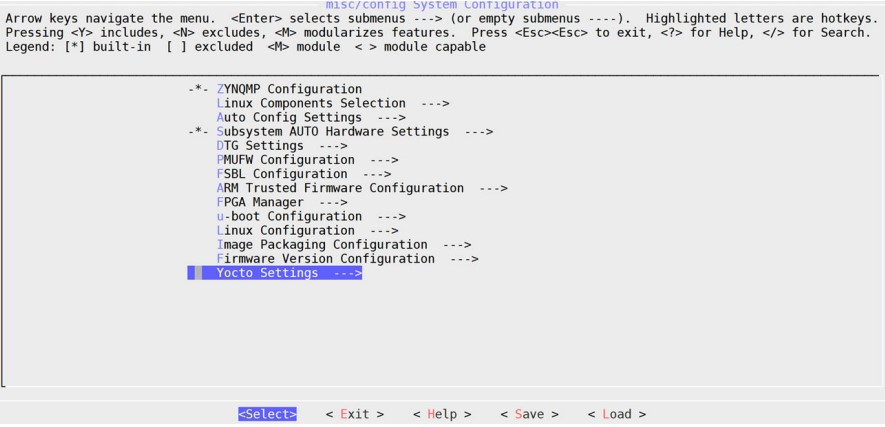
\includegraphics[width=0.9\textwidth]{images/image1.jpg}
\caption{Schermata di configurazione del sistema}
\end{figure}
Ai fini della tesi sarà necessario abilitare il parametro FPGA Manager, che trattato nel dettaglio al capitolo \ref{chap:Cap3}.\\
Dopo aver configurato l'hardware e quindi i parametri del boot loader\footnote{U-BOOT}, è necessario riconfigurare il file system ed eventualmente il kernel.
\begin{lstlisting}[language=sh, label=lst:FileSystem, caption={Comando necessario alla riconfigurazione del file system}]
petalinux-config -c rootfs

\end{lstlisting}
Se il comando è andato a buon fine comparirà la seguente schermata
\begin{figure}[h]
\centering
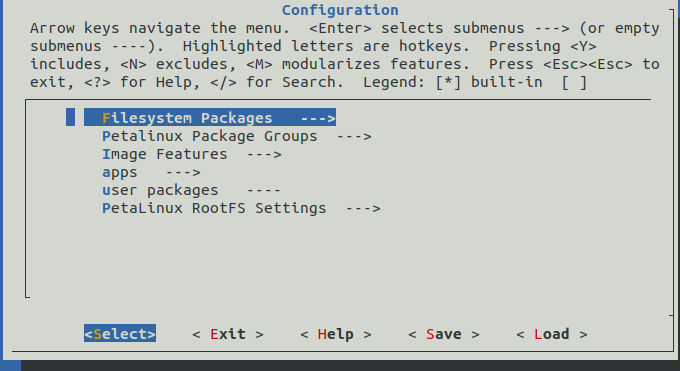
\includegraphics[width=0.9\textwidth]{images/peta1.png}
\caption{Schermata di modifica file system}
\end{figure}
Da qui sarà possibile attivare o disattivare packages, al fine della programmazione on-board e per un ottimale interfacciamento con il sistema cloud è fortemente consigliato abilitare i seguenti package:
\begin{itemize}
    \item \textit{Petalinux Package Groups -> packagegroup-petalinux-utils}, al fine di avere GCC per l'architettura ARM Cortex A9.
    \item \textit{Petalinux Package Groups -> packagegroup-petalinux-python} e \textit{Filesystem Packages-> devel-> Python}, al fine di avere l'interprete di Python.
    \item \textit{console-> utils -> git}, al fine di avere il comando git.
\end{itemize}
Terminato ciò si potrà passare alla modifica del kernel, questa modifica risulta necessaria per poter effettuare le attività di tesi.
\begin{lstlisting}[language=sh, label=lst:sh, caption={Comando necessario alla riconfigurazione del kernel}]
petalinux-config -c kernel
\end{lstlisting}
Dalla schermata, che sarà analoga a quelle precedenti, è necessario abilitare i seguenti moduli\footnote{Per "[*]" si intende selezionato e si fa posizionandosi sopra il modulo desiderato e premendo la barra spaziatrice}:
\begin{itemize}
    \item \textit{Device Drivers ---> FPGA Configuration Framework -> [*]FPGA Region}, l'FPGA Region verrà discussa nel dettaglio nel capitolo \ref{cap5}
    \item \textit{Device Drivers ---> FPGA Configuration Framework -> [*]FPGA Bridge Framework}, il Bridge verrà discusso nel dettaglio nel capitolo \ref{cap5}
    \item \textit{Device Drivers --> Device Tree and Open Firmware support -> [*] Device Tree Overlays}, il suo scopo è modificare il device tree del kernel mentre è in esecuzione, una sua modifica si ripercuote sul lato FPGA, causandone una modifica.
    \item \textit{Device Drivers --> Device Tree and Open Firmware support -> [*] Device Tree Overlays ConfigFS Interface}
    \item \textit{Memory Management options ---> [*] Contiguous Memory Allocator}, il Contiguous Memoy Allocator verrà discusso nel dettaglio nel capitolo \ref{comunicazioneCap}
    \item \textit{Library routines--> DMA Contiguous Memory Allocator }
\end{itemize}

\section{Creazione app e modulo kernel}
Creare un app a livello kernel può risultare comodo, al fine di creare l'applicazione ed innestarla al nostro file system sarà necessario eseguire il seguente comando:
\begin{lstlisting}[language=sh, label=lst:creazioneApp, caption={Comando necessario alla creazione dell'applicazione, va eseguito nella cartella del progetto}]
petalinux-create -t apps --name [nome desiderato] --template [c, c++, autoconf, install]
\end{lstlisting}
Se il comando è stato eseguito correttamente il codice per l'applicazione si troverà nella cartella 
\textit{/project-spec/meta-user/recipes-apps/Nome Desiderato}.
\subsection{Compilazione}
Prima di poter compilare l'applicazione sarà necessario aggiungerla al file system, eseguendo i comandi visti nel codice \ref{lst:FileSystem}, spostandoci nel menu \textit{apps -> [nome desiderato]} sarà possibile selezionarlo.\\
Effettuato ciò per compilare è necessario eseguire:
\begin{lstlisting}[language=sh, label=lst:sh, caption={Comando necessario alla compilazione dell'applicazione}]
petalinux-build -c [nome desiderato]
\end{lstlisting}
\subsection{Modulo kernel}
Ai fini della creazione del modulo per il kernle, sarà necessario eseguire alcuni comandi:
\begin{lstlisting}[language=sh, label=lst:sh, caption={Comando necessario alla creazione del modulo kernel}]
petalinux-create -t modules --name [nome desiderato] --enable
\end{lstlisting}
Analogalmente all'applicazione il modulo si troverà nella cartella \textit{/project-spec/meta-user/recipes-modules/[nome desiderato]}, esso sarà compilato una volta compilato il kernel.

\section{Compilazione kernel}
Una volta ultimata la progettazione e la configurazione del kernel e del file system è necessaria la compilazione al fine di generare il codice binario, in ambiente petalinux sarà necessario usare il comando
\begin{lstlisting}[language=sh, label=lst:sh, caption={Comando necessario alla compilazione del kernel}]
petalinux-build
\end{lstlisting}
Questo passaggio sarà onesoro temporalmente, poichè si dovranno linkare tutte le librerie ed eventualmente scaricare moduli aggiunti in fase di configurazione.
\subsection{Pacchettizzazione del kernel}
Una volta che il kernel è compilato nella cartella \textit{images/linux} si troveranno tutte le componenti del sistema operativo. Quindi eseguendo il seguente comando
\begin{lstlisting}[language=sh, label=lst:sh, caption={Comando necessario alla pacchettizzazione del kernel}]
petalinux-package -boot -format BIN -fsbl image/linux/[FSBL] -fpga <path/to/bitstream> -u-boot
\end{lstlisting}
